%%%%%%%%%%%%%%%%%%%%%%%%%%%%%%%%%%%%%%%%%%%%%%%%%%%%%%%%%%%%%%
% --> INTRODUCCIÓN
%%%%%%%%%%%%%%%%%%%%%%%%%%%%%%%%%%%%%%%%%%%%%%%%%%%%%%%%%%%%%%
\section{Introducción}

Se denomina tiempo de compilación (\textit{compile-time} en inglés) al intervalo de tiempo en el que un compilador compila código escrito en un lenguaje de programación a una forma de código ejecutable por una máquina.

El compilador normalmente realiza un chequeo de sintaxis, que incluye entre otros un chequeo de tipos y ejecución de reglas de ámbito, seguido de un análisis semántico, que se compone de procesos como el enlazado estático, la instanciación de plantillas y la optimización del código generado. El enlazado dinámico se realiza normalmente después del tiempo de compilación, bien en tiempo de ejecución o antes de éste, por medio de un cargador de programas. El chequeo de límites de arrays normalmente no se hace en tiempo de compilación. \cite{R1}
%%%%%%%%%%%%%%%%%%%%%%%%%%%%%%%%%%%%%%%%%%%%%%%%%%%%%%%%%%%%%%
% --> OBJETIVOS
%%%%%%%%%%%%%%%%%%%%%%%%%%%%%%%%%%%%%%%%%%%%%%%%%%%%%%%%%%%%%%
\subsection{Objetivos}



%%%%%%%%%%%%%%%%%%%%%%%%%%%%%%%%%%%%%%%%%%%%%%%%%%%%%%%%%%%%%%
% --> OBJETIVO GENERAL
%%%%%%%%%%%%%%%%%%%%%%%%%%%%%%%%%%%%%%%%%%%%%%%%%%%%%%%%%%%%%%
\subsubsection{Objetivo General}
\begin{itemize}
\item Medir tiempo de compilación de programas desarrollados en ciertos programas.
\end{itemize}

%%%%%%%%%%%%%%%%%%%%%%%%%%%%%%%%%%%%%%%%%%%%%%%%%%%%%%%%%%%%%%
% --> OBJETIVOS ESPECÍFICOS
%%%%%%%%%%%%%%%%%%%%%%%%%%%%%%%%%%%%%%%%%%%%%%%%%%%%%%%%%%%%%%
\subsubsection{Objetivos Específicos}
\begin{itemize}
\item Calcular tiempo de ejecución de lectura y de suma de datos de un programa en Python.
\item Calcular tiempo de ejecución de lectura y de suma de datos de un programa en C.
\item Calcular tiempo de ejecución de lectura y de suma de datos de un programa en C++.
\item Calcular tiempo de ejecución de lectura y de suma de datos de un programa en Java.
\end{itemize}

%%%%%%%%%%%%%%%%%%%%%%%%%%%%%%%%%%%%%%%%%%%%%%%%%%%%%%%%%%%%%%
% --> ENUNCIADO
%%%%%%%%%%%%%%%%%%%%%%%%%%%%%%%%%%%%%%%%%%%%%%%%%%%%%%%%%%%%%%
%\newpage

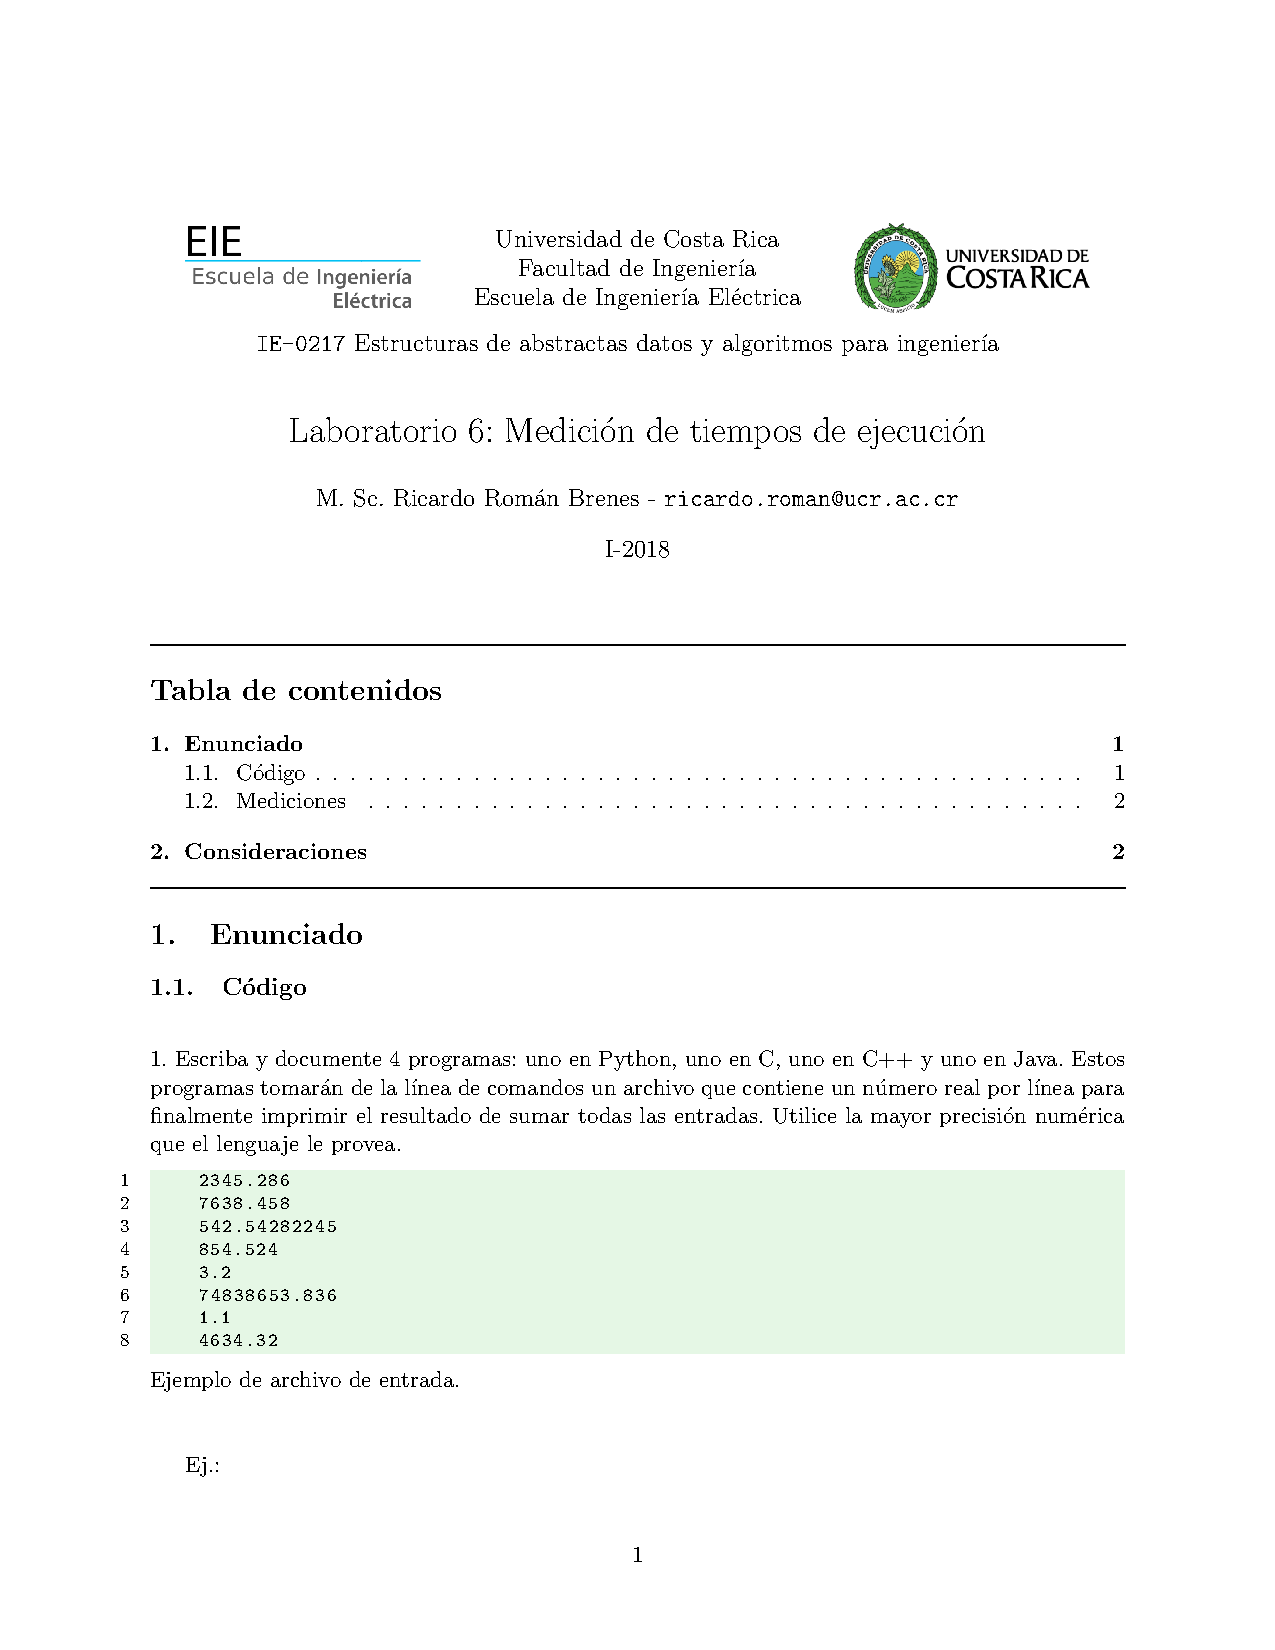
\includepdf[pages=1,pagecommand=\section{Enunciado}, scale=0.8]{enunciados/enun6} 
\includepdf[pages=2,pagecommand={},scale=0.8]{enunciados/enun6}

%%%%%%%%%%%%%%%%%%%%%%%%%%%%%%%%%%%%%%%%%%%%%%%%%%%%%%%%%%%%%%
% --> SOLUCIÓN
%%%%%%%%%%%%%%%%%%%%%%%%%%%%%%%%%%%%%%%%%%%%%%%%%%%%%%%%%%%%%%
\section{Solución}
%%%%%%%%%%%%%%%%%%%%%%%%%%%%%%%%%%%%%%%%%%%%%%%%%%%%%%%%%%%%%%
% --> PYTHON
%%%%%%%%%%%%%%%%%%%%%%%%%%%%%%%%%%%%%%%%%%%%%%%%%%%%%%%%%%%%%%
\subsection{Solución Python}
Para calcular los tiempos que tarda Python en ejecutar la apertura del archivo y la suma de los valores de este, se utiliza la biblioteca \texttt{timeit} que contiene la función \texttt{default\_timer}. Esta función retorna el tiempo de ejecución hasta el momento que se ejecuta, en milisegundos. Llamando la función antes y después de se realicen las operaciones necesarias se puede calcular la diferencia entre las mediciones, esto es, el tiempo que tardó en ejecutarse este fragmento de código.
\begin{minted}[linenos,autogobble,bgcolor=bg,breaklines,fontsize=\footnotesize ]{python}
# -*- coding: utf-8 -*-
from timeit import default_timer as timer
import sys
def leerArchivo():
	lista = []
	ruta = sys.argv[1]
	with open(ruta,'r') as file:
		for line in file:
			lista.append(line)
	return lista
def sumar(lista):
	total = 0
	for elemento in lista:
		total += float(elemento)
	return total
if __name__ == "__main__":
	print ("\n**** Compilación de Python ****")
	t0 = timer()
	data = leerArchivo()
	t1 = timer()
	sumar(data)
	t2 = timer()
	print("Tiempo de la lectura de datos: ","%.12f "%((t1-t0)*1000), "ms")
	#print(t1-t0)
	print("Tiempo de la suma de datos: ", "%.12f "%((t2-t1)*1000), "ms")
	print(sumar(data))
	#print(leerArchivo())

\end{minted}

%%%%%%%%%%%%%%%%%%%%%%%%%%%%%%%%%%%%%%%%%%%%%%%%%%%%%%%%%%%%%%
% --> C
%%%%%%%%%%%%%%%%%%%%%%%%%%%%%%%%%%%%%%%%%%%%%%%%%%%%%%%%%%%%%%
\subsection{Solución C}

Para medir el tiempo de ejecución en \texttt{C} se utiliza la función \texttt{clock()} de la biblioteca \texttt{time.h}, esta función tiene la peculiaridad de que devuelve los pulsos (\textit{ticks}) del reloj desde que se ejecutó el programa, por esto se debe dividir el resultado entre \texttt{CLOCKS\_PER\_SEC}, que es la cantidad de pulsos de reloj del equipo. Una vez se realiza esta operación se obtiene el resultado en segundos.

\begin{minted}[linenos,autogobble,bgcolor=bg,breaklines,fontsize=\footnotesize ]{c}
#include <stdio.h>
#include <stdlib.h>
#include <time.h>

int main(int argc, char const *argv[])
{
  printf("\n****** Compilación de C ******\n");
  char const * filename = argv[1];
  clock_t timeInit, timeEnd;
  long double seconds;

  // Abriendo archivo de datos
  FILE *archivo;
  archivo = fopen(filename, "r");

  if (!archivo)
  {
      printf("No se pudo abrir el archivo: ../input/in.data\n");
      exit(1);
  }

  // Obtiene tamano de la cantidad de datos de entrada
  int count = 0;
  char str[60];
  while (fgets(str,60,archivo)!=NULL) count++;

  // Lectura del archivo
  archivo = fopen(filename, "r");
  long double dataArray[count];
  int i = 0;
  timeInit = clock();
  while (fgets(str,60,archivo)!=NULL)
  {
     dataArray[i]= (long double)atof(str);
     i++;
  }
  timeEnd = clock();
  seconds = (double)(timeEnd - timeInit) / CLOCKS_PER_SEC; /*según que estes midiendo el tiempo en segundos es demasiado grande*/
  printf("Tiempo de la lectura de datos: %Lf s\n",seconds);


  // Suma de los datos del archivo
  long double sumResult = 0;
  timeInit = clock();
  for(int i = 0; i<count; i++) sumResult += dataArray[i];
  timeEnd = clock();
  seconds = (double)(timeEnd - timeInit) / CLOCKS_PER_SEC; /*según que estes midiendo el tiempo en segundos es demasiado grande*/
  printf("Tiempo de la suma de datos: %Lf s \n",seconds);

  // Imprime resultado
  printf("%Lf\n",sumResult);
  // Cerrando archivo
  fclose(archivo);
  return 0;
}
\end{minted}

%%%%%%%%%%%%%%%%%%%%%%%%%%%%%%%%%%%%%%%%%%%%%%%%%%%%%%%%%%%%%%
% --> C++
%%%%%%%%%%%%%%%%%%%%%%%%%%%%%%%%%%%%%%%%%%%%%%%%%%%%%%%%%%%%%%
\subsection{Solución C++}

En \texttt{C++} se cuenta con la biblioteca \texttt{chrono} para medir el tiempo de ejecución. Con la instrucción \texttt{chrono::high\_resolution\_clock::now()} se crea un marcador o \textit{timepoint} en el punto deseado, con esto se calcula la duración en milisegundos de cada segmento de interés. 

\begin{minted}[linenos,autogobble,bgcolor=bg,breaklines,fontsize=\footnotesize ]{c++}
#include <iostream>
#include <string>
#include <fstream>
#include <vector>
#include <chrono>
using namespace std;


long double sum(int array_size, long double * data){
	long double total=0.0;
	for (int i=0; i<array_size; i++){
		total+=data[i];
	}
	return total;
}

int main(int argc, char const *argv[]){
	
	cout << "\n***** Compilación de C++ *****"<<endl;
	const char* path = argv[1];
	
	//Se hace un timepoint antes de abrir archivo
	auto t0 = chrono::high_resolution_clock::now();
	
	fstream file(path,ios::in);
	string line;
	int arr_size = 0;
	int counter = 0;
	long double x = 0.0;
	//contar cantidad de líneas, = tamaño del array
	if (file.is_open()){
		while(getline(file,line)){
			arr_size++;
		}
		file.close();
		
	}
	else{
		cout << "Unable to open file!" << endl;
		exit(0);
	}
		
	//asignación de valores a elementos del array	
	long double *data = new long double[arr_size];
	line = "";
	file.open(path);
	while(getline(file,line)){
		x = stold(line);
		data[counter] = x;
		counter++;
	}
	file.close();
	
	//otro timepoint antes de sumar los datos del arreglo
	auto t1 = chrono::high_resolution_clock::now();
	long double suma = sum(arr_size, data);
	auto t2 = chrono::high_resolution_clock::now();
	
	chrono::duration<double> tFileOpen = t1 - t0;
	chrono::duration<double> tSumData = t2 - t1;

	cout << fixed << endl << "La suma da " << suma << endl;
	cout << "---------------------------------------------------------" << endl;
	cout << "Tiempo de la lectura de datos: " << (tFileOpen.count()*1000) << " ms" << endl;
	cout << "Tiempo de la suma de datos: " << (tSumData.count()*1000) << " ms" << endl;

	delete data;
	return 0;
}
\end{minted}

%%%%%%%%%%%%%%%%%%%%%%%%%%%%%%%%%%%%%%%%%%%%%%%%%%%%%%%%%%%%%%
% --> JAVA
%%%%%%%%%%%%%%%%%%%%%%%%%%%%%%%%%%%%%%%%%%%%%%%%%%%%%%%%%%%%%%
\subsection{Solución Java}

En \texttt{Java} se utiliza la función \texttt{System.currentTimeMillis()} para obtener el tiempo desde la ejecución hasta el punto deseado, poniendo estos puntos antes y después, se puede calcular el tiempo de ejecución. Es importante destacar que esta función devuelve la cantidad de milisegundos en un dato tipo \texttt{long} debido a la gran precisión que brinda, por lo que se deben inicializar las variables para medir utilizando este tipo de dato.

\begin{minted}[linenos,autogobble,bgcolor=bg,breaklines,fontsize=\footnotesize ]{java}

import java.io.*;

public class suma
{
  public static void main(String[] args)throws Exception
  {
    long time_start1, time_end1, time_start2, time_end2;

    System.out.println("\n***** Compilación de Java *****");

    time_start1 = System.currentTimeMillis();
    System.out.println("Start: " +(time_start1)+ "ms");
    File file = new File(args[0]);
    BufferedReader br = new BufferedReader(new FileReader(file));
    String st;

    // Obtiene tamano de la cantidad de datos de entrada
    int i = 0;
    while ((st = br.readLine()) != null) i++;

    // Lectura del archivo
    double dataArray[] = new double [i];
    int count = 0;
    br = new BufferedReader(new FileReader(file));


    while ((st = br.readLine()) != null)
    {
      dataArray[count] = Double.parseDouble(st);
      count++;
    }
    time_end1 = System.currentTimeMillis();
    System.out.println("End: " +(time_end1)+ "ms");
    System.out.println("Tiempo de la lectura de datos: " + (time_end1-time_start1)+ "ms");

    // Suma de los datos del archivo
    double sumaResult = 0;
    time_start2 = System.currentTimeMillis();
    //BigDecimal t3 = new BigDecimal( System.currentTimeMillis() );
    for (int j = 0; j<count; j++) sumaResult+=dataArray[j];
    time_end2 = System.currentTimeMillis();
    //BigDecimal t4 = new BigDecimal( System.currentTimeMillis() );

    System.out.println("Tiempo de la suma de datos: " +(time_end1-time_start1)+ "ms");

    System.out.printf("Resultado de la suma: %f\n",sumaResult);

  }
}


\end{minted}

%%%%%%%%%%%%%%%%%%%%%%%%%%%%%%%%%%%%%%%%%%%%%%%%%%%%%%%%%%%%%%
% --> RESULTADOS
%%%%%%%%%%%%%%%%%%%%%%%%%%%%%%%%%%%%%%%%%%%%%%%%%%%%%%%%%%%%%%
\section{Resultados}

Para este laboratorio se realizaron varias pruebas para determinar los distintos tiempos de ejecución de acuerdo al lenguaje utilizado. En la Tabla \ref{chart} se muestran los resultados para cada una de las seis veces que se ejecutó el código de cada lenguaje; además, en las Figuras \ref{fig:C}, \ref{fig:C++}, \ref{fig:Py}, y \ref{fig:Java} se muestran los mismos resultados pero según como se observan en la terminal, y también se aprecia cómo se envía o indica al programa el archivo que debe leer en donde se encuentra la información. 

Como era de esperar, el lenguaje más rápido de todos fue \texttt{C}, seguido por \texttt{C++}. Estos dos lenguajes son compilados, es decir, primero se compila el código y luego la máquina lo ejecuta, entre sus ventajas se encuentra precisamente el tiempo de ejecución, el cuál es mucho mejor que el de los lenguajes interpretados como \texttt{Python} o \texttt{Java}. Si se observa nuevamente la Tabla \ref{chart} se puede notar que los tiempos están dados en microsegundos, esto porque son los tiempos manejados por C. En contraste a lo anterior, se nota que Java tarda mucha más en ejecutarse, aproximadamente $1000 \mu s$, es decir, un milisegundo. Esto es mucho mayor que el tiempo de C o C++, pero también es importante notar lo consistente de este resultado, el cual se mantuvo constante, a diferencia de los demás lenguajes en donde sí hubo una variación considerable entre los valores obtenidos. En la Figura \ref{fig:chart} se puede observar gráficamente los resultados obtenidos y comentados anteriormente.

\begin{table}[]
\centering
\caption{Resultados ejecución de los códigos.}
\label{chart}
\begin{tabular}{lrr}
Lenguaje                & Tiempo de lectura ($\mu$s) & Tiemp de suma ($\mu$s) \\
                        &                       &                   \\
\multirow{6}{*}{C}      & 28                    & 1                 \\
                        & 15                    & 1                 \\
                        & 13                    & 1                 \\
                        & 15                    & 0                 \\
                        & 39                    & 2                 \\
                        & 39                    & 2                 \\
Promedio                & 24.83333333           & 1.166666667       \\
                        &                       &                   \\
\multirow{6}{*}{C++}    & 50.27                 & 0.16              \\
                        & 49.85                 & 0.13              \\
                        & 189.71                & 0.47              \\
                        & 53.77                 & 0.12              \\
                        & 53.64                 & 0.17              \\
                        & 153.57                & 0.5               \\
Promedio                & 91.80166667           & 0.2583333333      \\
                        &                       &                   \\
\multirow{6}{*}{Java}   & 1000                  & 1000              \\
                        & 1000                  & 1000              \\
                        & 1000                  & 1000              \\
                        & 1000                  & 1000              \\
                        & 1000                  & 1000              \\
                        & 1000                  & 1000              \\
Promedio                & 1000                  & 1000              \\
                        &                       &                   \\
\multirow{6}{*}{Python} & 23.13                 & 16.93             \\
                        & 31.95                 & 23.13             \\
                        & 31.95                 & 22.89             \\
                        & 20.03                 & 15.02             \\
                        & 25.99                 & 18.83             \\
                        & 42.91                 & 30.04             \\
Promedio                & 29.32666667           & 21.14            
\end{tabular}
\end{table}

\begin{figure}[H]
\centering
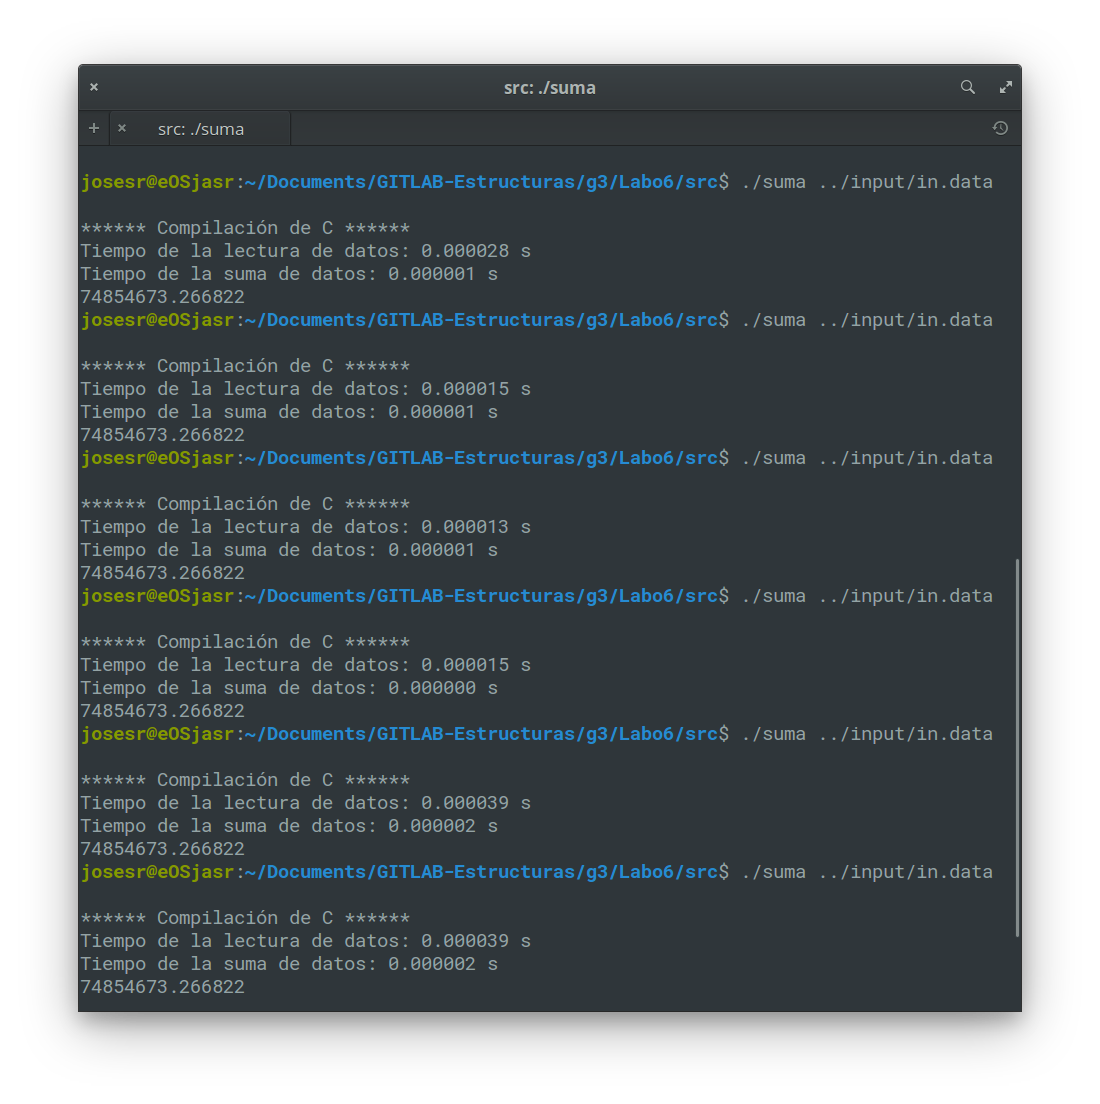
\includegraphics[width=\textwidth]{imgs/Labo6/resC.png}
\caption{Ejecución del código de \texttt{C}.}
\label{fig:C}
\end{figure}

\begin{figure}[H]
\centering
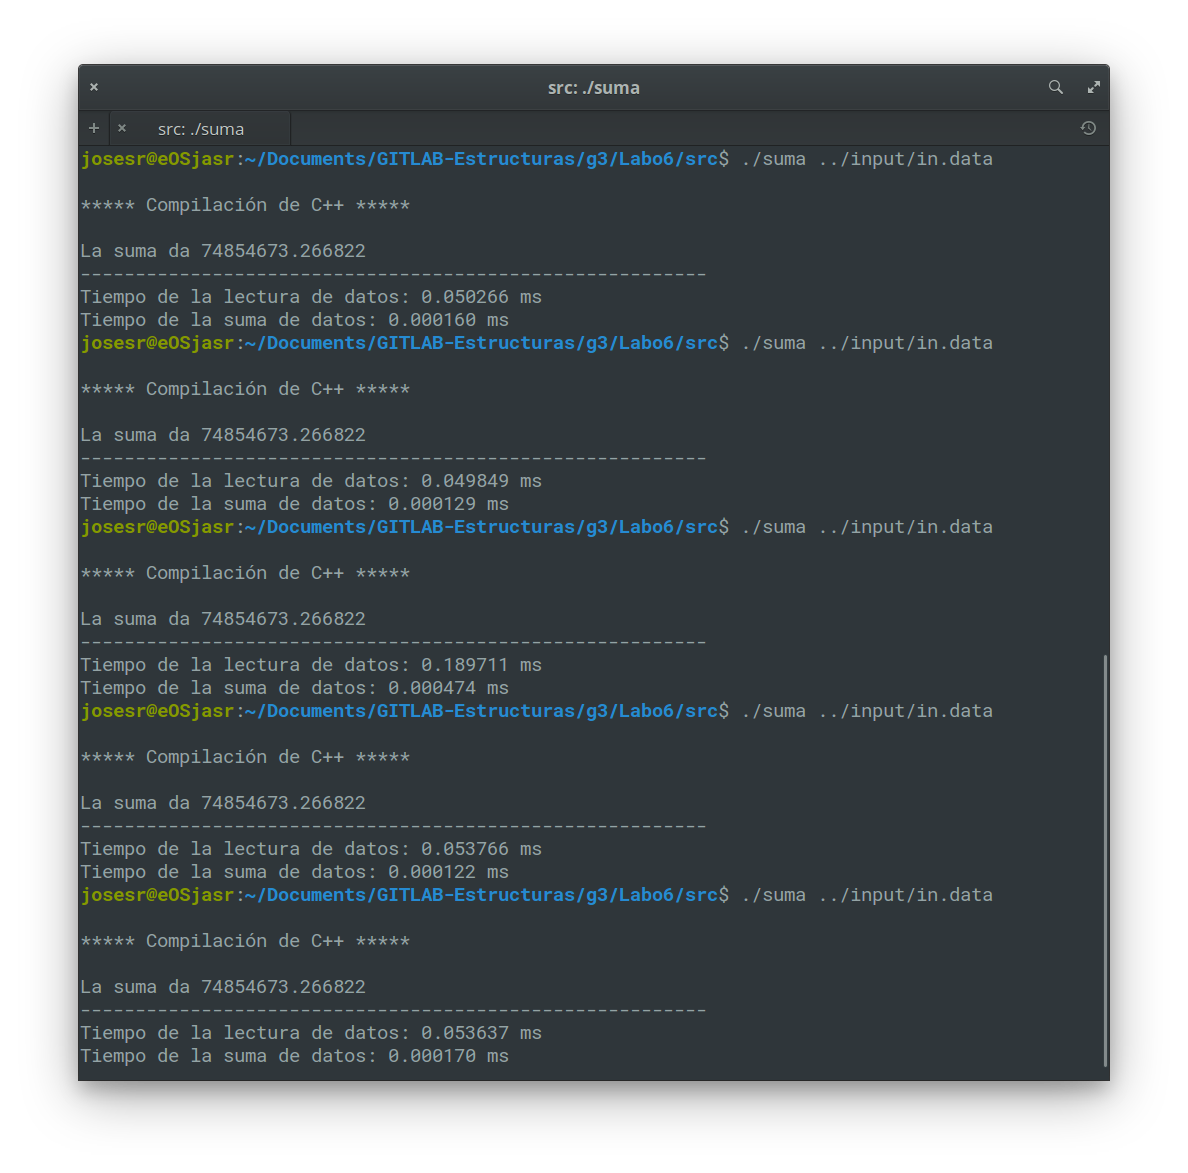
\includegraphics[width=\textwidth]{imgs/Labo6/resCPP.png}
\caption{Ejecución del código de \texttt{C++}.}
\label{fig:C++}
\end{figure}

\begin{figure}[H]
\centering
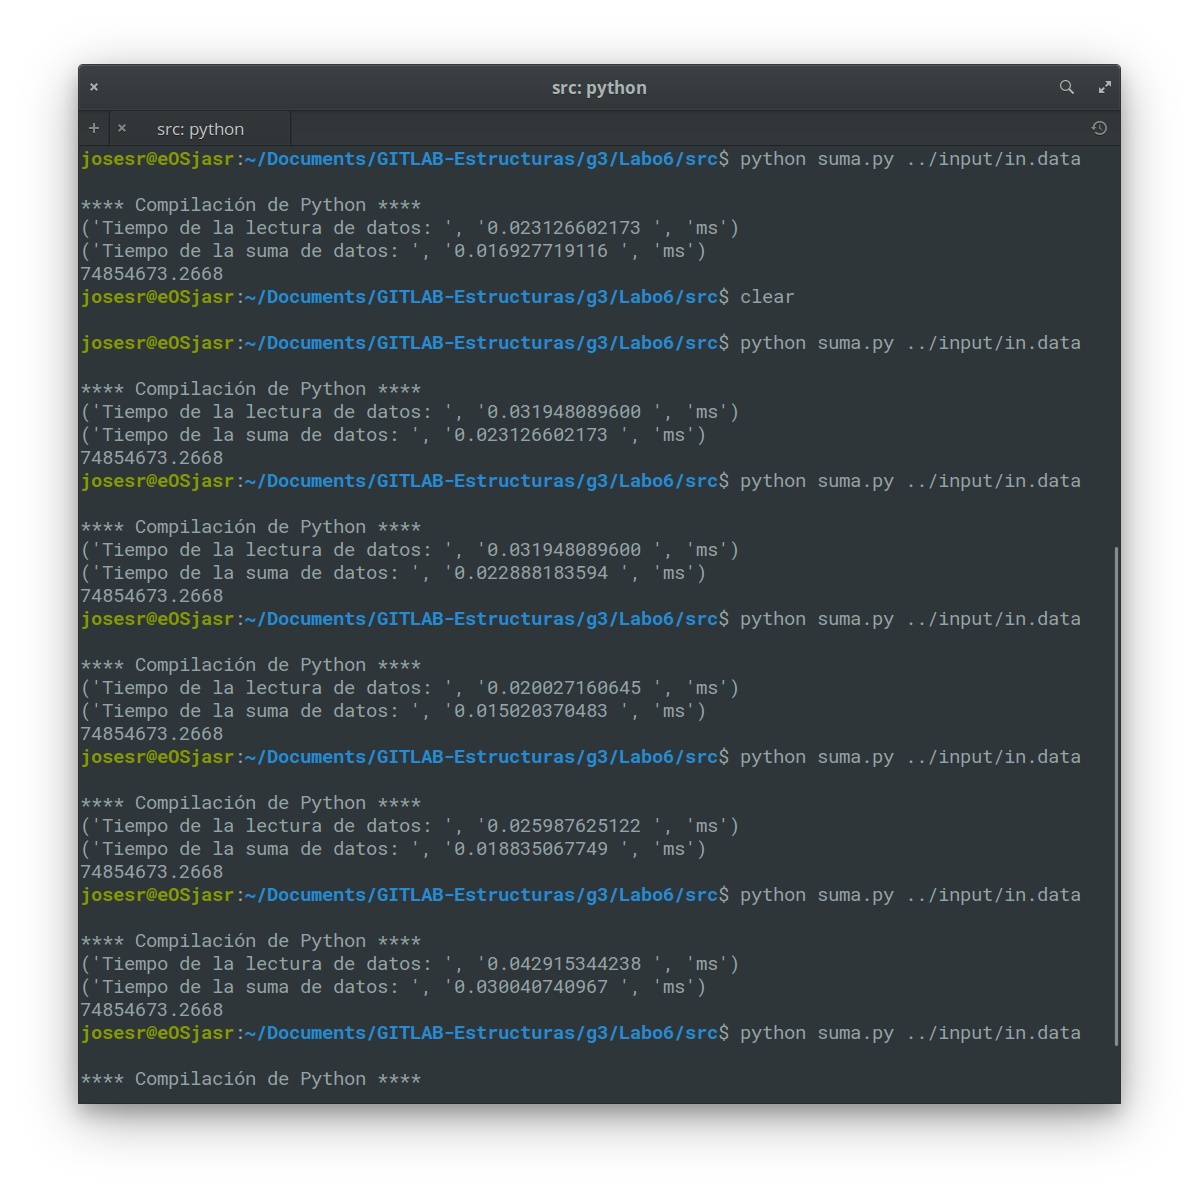
\includegraphics[width=\textwidth]{imgs/Labo6/resPY.png}
\caption{Ejecución del código de \texttt{Python}.}
\label{fig:Py}
\end{figure}

\begin{figure}[H]
\centering
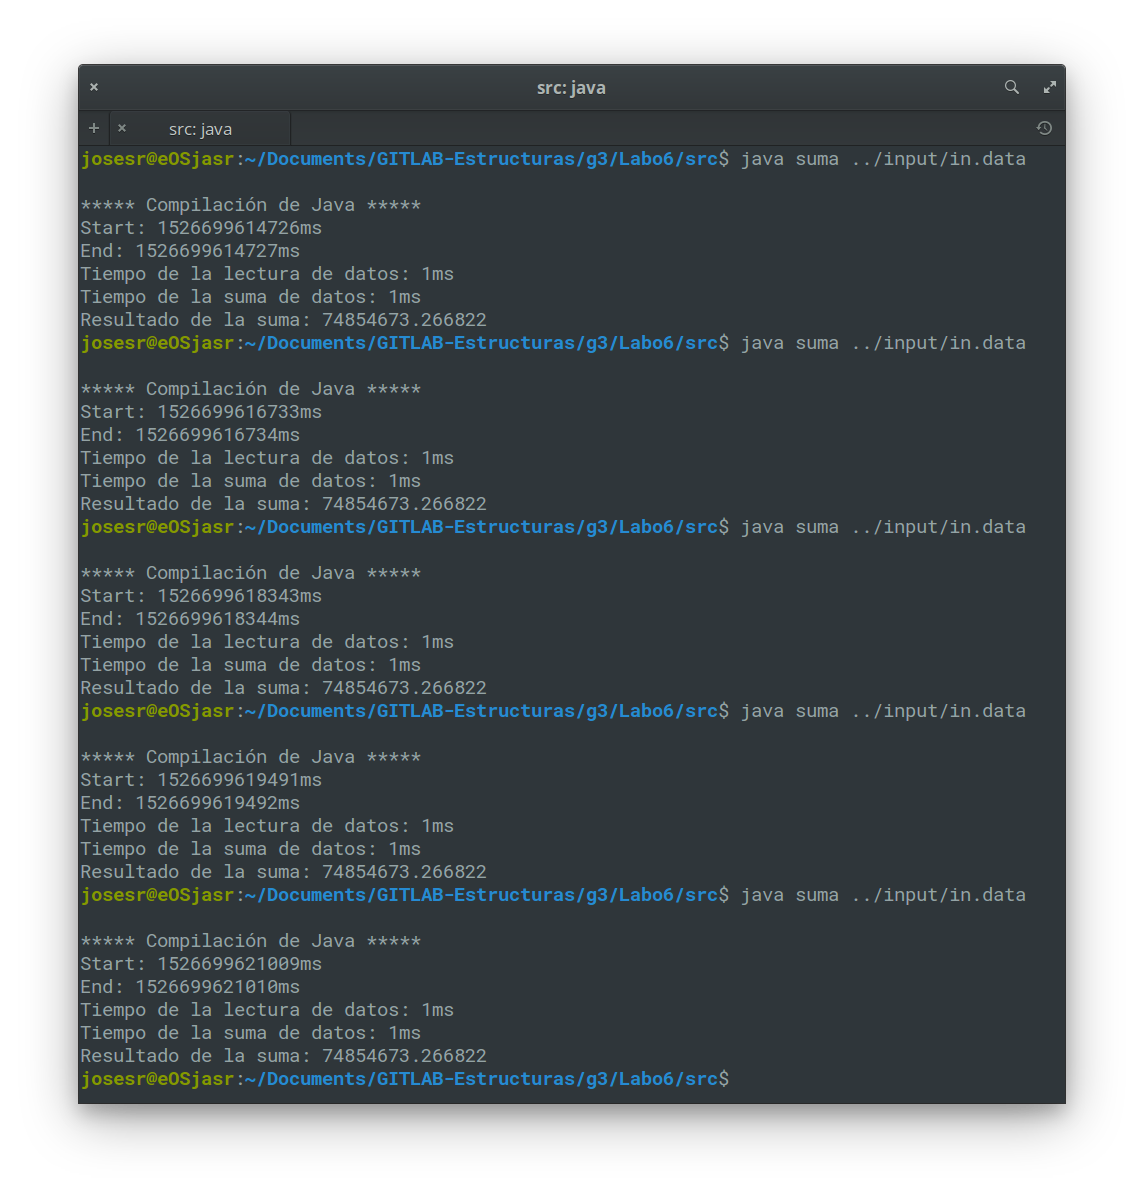
\includegraphics[width=\textwidth]{imgs/Labo6/resJAVA.png}
\caption{Ejecución del código de \texttt{Java}.}
\label{fig:Java}
\end{figure}

\begin{figure}[H]
\centering
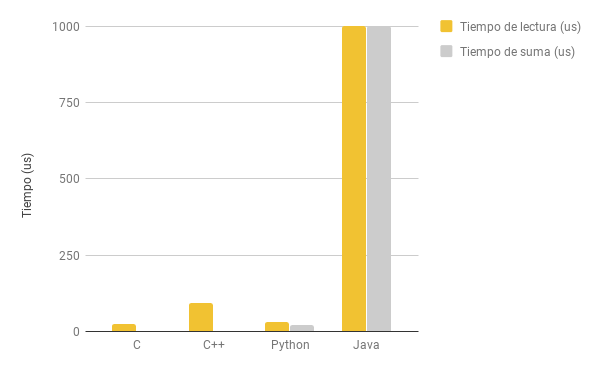
\includegraphics[width=\textwidth]{imgs/Labo6/chart.png}
\caption{Comparación de los tiempos para los cuatro lenguajes utilizados.}
\label{fig:chart}
\end{figure}

%%%%%%%%%%%%%%%%%%%%%%%%%%%%%%%%%%%%%%%%%%%%%%%%%%%%%%%%%%%%%%
% --> CONCLUSIONES
%%%%%%%%%%%%%%%%%%%%%%%%%%%%%%%%%%%%%%%%%%%%%%%%%%%%%%%%%%%%%%
\section{Conclusiones}

Como conclusiones se tiene que:
\begin{itemize}
\item El lenguaje C es el más rápido de todos.
\item Los lenguajes compilados (C, C++) son mucho más rápidos que los lenguajes interpretados (Java, Python).
\item EL lenguaje Java es mucho más lento que los demás.
\item Hay diversas formas de medir el tiempo de ejecución que pueden presentar mejor o peor 
\end{itemize}


%%%%%%%%%%%%%%%%%%%%%%%%%%%%%%%%%%%%%%%%%%%%%%%%%%%%%%%%%%%%%%
% --> BIBLIOGRAFIA
%%%%%%%%%%%%%%%%%%%%%%%%%%%%%%%%%%%%%%%%%%%%%%%%%%%%%%%%%%%%%%
\begin{thebibliography}{IEEE}
\bibitem{R1} Talens, S. \textbf{\textit{Curso de programación en C++}}. EUI (UPV) Valencia, 17 al 28 de Julio de 1995. 

\bibitem{R2} Raffo, E. \textbf{\textit{Programación genérica en C++, usando Metaprogramación}}. 2007. Sistemas de Informática. 
\end{thebibliography}

